\documentclass[border=10pt]{standalone}
\usepackage[svgnames]{xcolor}
\usepackage{amsmath}
\usepackage{pgfplots}
\pgfplotsset{compat=newest}
\usepackage[sfdefault]{FiraSans}
\usepackage{FiraMono}
\renewcommand*\familydefault{\sfdefault}
\begin{document}
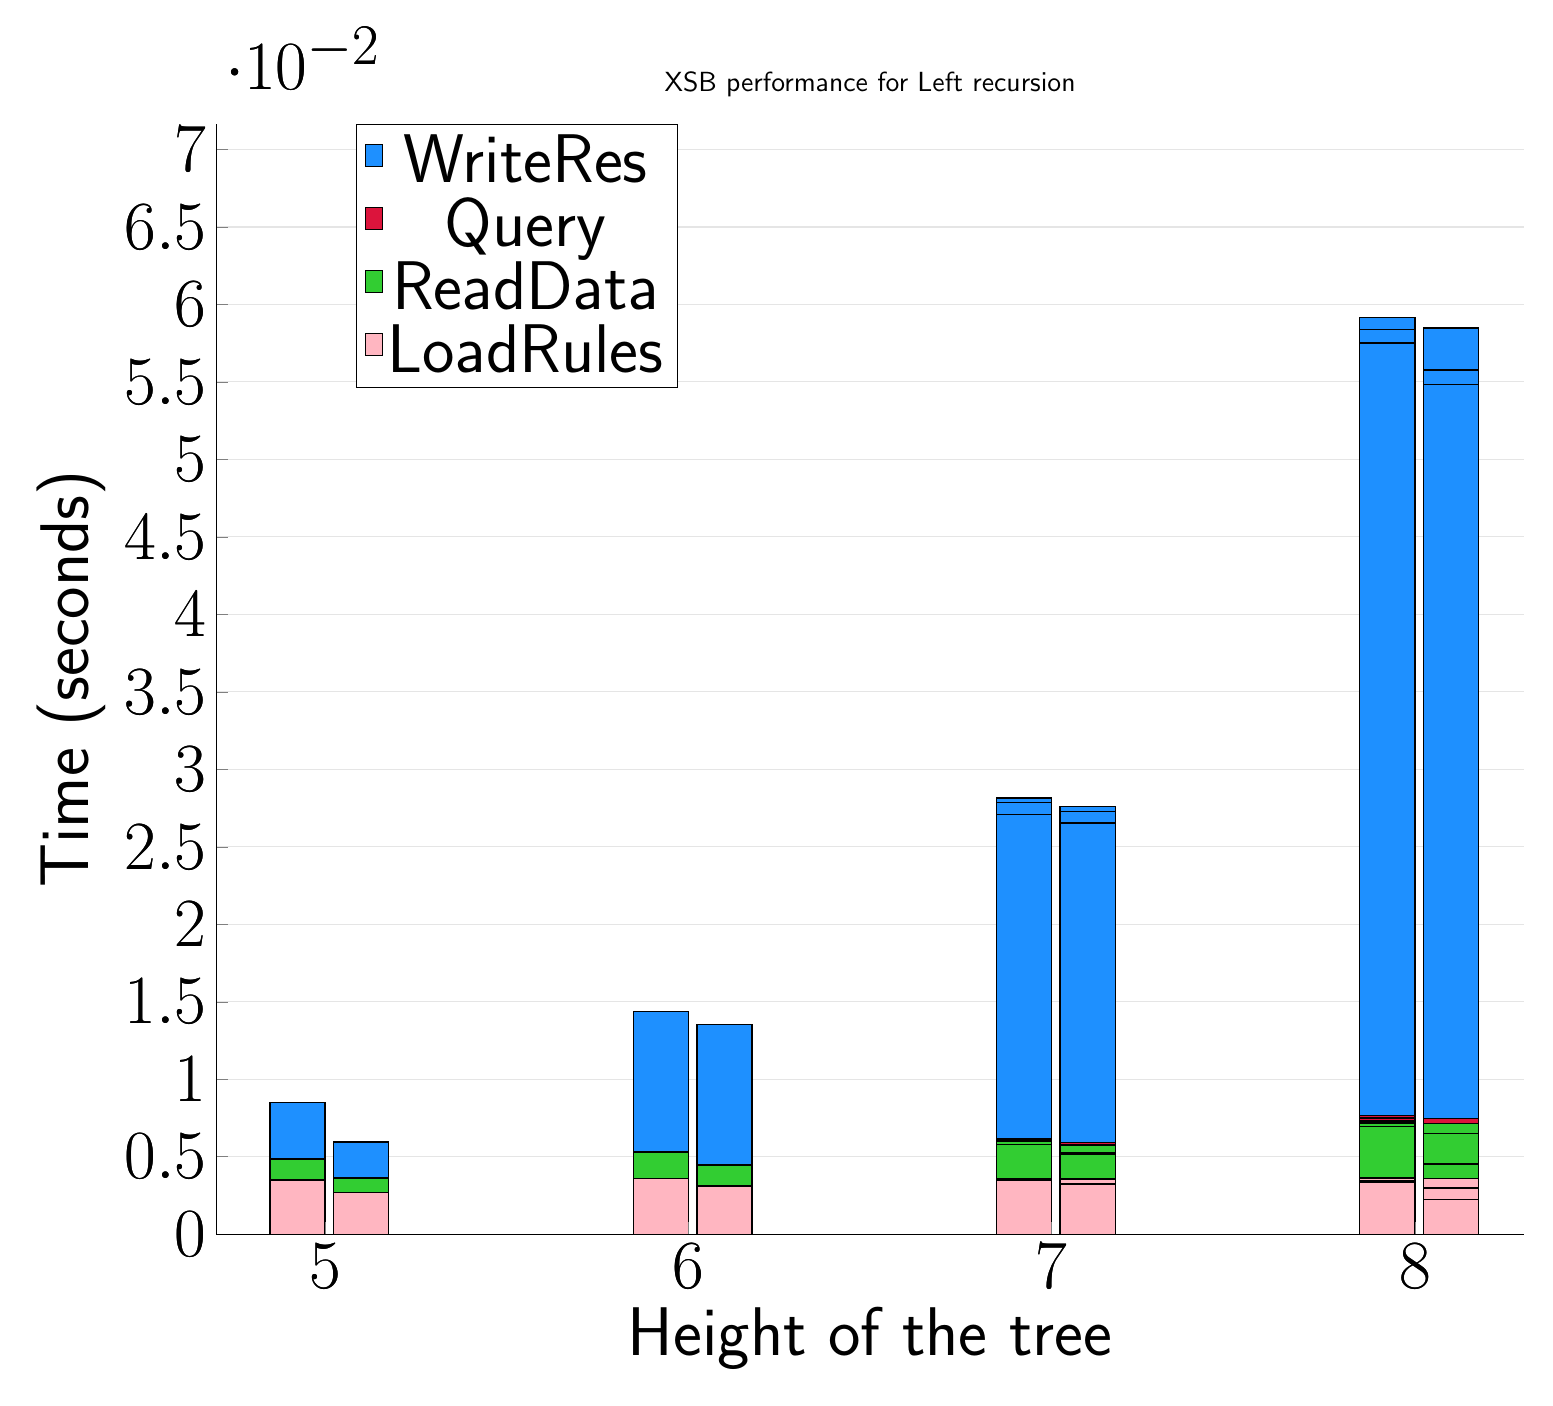
\begin{tikzpicture}
\begin{axis}[
   ybar stacked,
   title={XSB performance for Left recursion},
   bar shift=-10pt,
   width=1.5\textwidth,
   bar width=0.7cm,
   ymajorgrids, tick align=inside,
   major grid style={draw=gray!20},
   xtick=data,
   ymin=0, ymax=0.07167722702026368,
   axis x line*=bottom,
   axis y line*=left,
   enlarge x limits=0.1,
   legend style={
       at={(0.23, 1)},
       anchor=north,
       legend columns=1,
       font=\Huge,
   },
   ylabel={Time (seconds)},
   xlabel={Height of the tree},
   label style={font=\Huge},
   tick label style={font=\Huge},
]
\addlegendimage{fill=DodgerBlue, draw=black, line width=0.2pt}
\addlegendentry{WriteRes}
\addlegendimage{fill=Crimson, draw=black, line width=0.2pt}
\addlegendentry{Query}
\addlegendimage{fill=LimeGreen, draw=black, line width=0.2pt}
\addlegendentry{ReadData}
\addlegendimage{fill=LightPink, draw=black, line width=0.2pt}
\addlegendentry{LoadRules}
\addplot +[fill=LightPink, draw=black, line width=0.5pt] coordinates {
    (5, 0.0035087267557779938)
    (6, 0.0035770734151204433)
    (7, 0.0035645961761474596)
    (7, 0.0036025842030843135)
    (7, 0.0034796396891276036)
    (8, 0.003431320190429687)
    (8, 0.0036292870839436868)
    (8, 0.003358920415242513)
};
\addplot +[fill=LimeGreen, draw=black, line width=0.5pt] coordinates {
    (5, 0.0012943744659423848)
    (6, 0.0016916592915852868)
    (7, 0.0024086634318033835)
    (7, 0.00241573651631673)
    (7, 0.0023206869761149065)
    (8, 0.0037503242492675764)
    (8, 0.003685951232910153)
    (8, 0.003606716791788737)
};
\addplot +[fill=Crimson, draw=black, line width=0.5pt] coordinates {
    (5, 3.9974848429362004e-05)
    (6, 6.858507792154946e-05)
    (7, 0.00014535586039225268)
    (7, 0.00014122327168782534)
    (7, 0.000137646993001302)
    (8, 0.00031868616739908867)
    (8, 0.00034173329671223973)
    (8, 0.00033132235209147137)
};
\addplot +[fill=DodgerBlue, draw=black, line width=0.5pt] coordinates {
    (5, 0.0036753018697102875)
    (6, 0.009044726689656573)
    (7, 0.02172470092773438)
    (7, 0.02199403444925944)
    (7, 0.0211319923400879)
    (8, 0.05167722702026368)
    (8, 0.05072522163391116)
    (8, 0.0502164363861084)
};
\end{axis}
\begin{axis}[
   ybar stacked,
   bar shift=13pt,
   width=1.5\textwidth,
   bar width=0.7cm,
   ymajorgrids, tick align=inside,
   major grid style={draw=none},
   xtick=data,
   ymin=0, ymax=0.07167722702026368,
   axis x line*=none,
   axis y line*=none,
   enlarge x limits=0.1,
   label style={font=\Huge},
   tick label style={font=\Huge},
]
\addplot +[fill=LightPink, draw=black, line width=0.5pt] coordinates {
    (5, 0.0027089999999999966)
    (6, 0.0031123333333333333)
    (7, 0.003565)
    (7, 0.003198666666666667)
    (7, 0.0032556666666666667)
    (8, 0.0029706666666666666)
    (8, 0.0035943333333333335)
    (8, 0.0022596666666666668)
};
\addplot +[fill=LimeGreen, draw=black, line width=0.5pt] coordinates {
    (5, 0.000900333333333332)
    (6, 0.001333)
    (7, 0.002190000000000003)
    (7, 0.001982666666666667)
    (7, 0.0020286666666666634)
    (8, 0.0035123333333333304)
    (8, 0.0035373333333333333)
    (8, 0.0022686666666666667)
};
\addplot +[fill=Crimson, draw=black, line width=0.5pt] coordinates {
    (5, 3.0333333333335932e-05)
    (6, 5.933333333333254e-05)
    (7, 0.00014433333333333168)
    (7, 0.00012666666666666593)
    (7, 0.00012800000000000298)
    (8, 0.000317333333333334)
    (8, 0.0003413333333333347)
    (8, 0.00022400000000000198)
};
\addplot +[fill=DodgerBlue, draw=black, line width=0.5pt] coordinates {
    (5, 0.002318666666666664)
    (6, 0.009039666666666666)
    (7, 0.021722)
    (7, 0.021959333333333334)
    (7, 0.02112133333333333)
    (8, 0.05167966666666666)
    (8, 0.04830466666666666)
    (8, 0.05009933333333333)
};
\end{axis}
\end{tikzpicture}

\end{document}
